TGC's provide two functions in the MS end-cap region\@: fast muon triggering ability and the measurement of the azimuthal coordinate to complement the precise radial measurements of the MDT's. Covering the pseudorapidity range of $1.05 < |\eta| < 2.4$, the TGC's are arranged in seven detector layers that sandwich the MDT chambers. Each TGC consists of several gas volumes that contain a wire plane and two cathode planes, which is referred to as a chamber. The seven detector layers are grouped into a triplet (three chambers) layer and two doublet (two chambers) layers, which are referred to as a unit. These can be seen in Figure~\ref{fig:tgc_chamber}

\begin{figure}[htp]
    \centering
    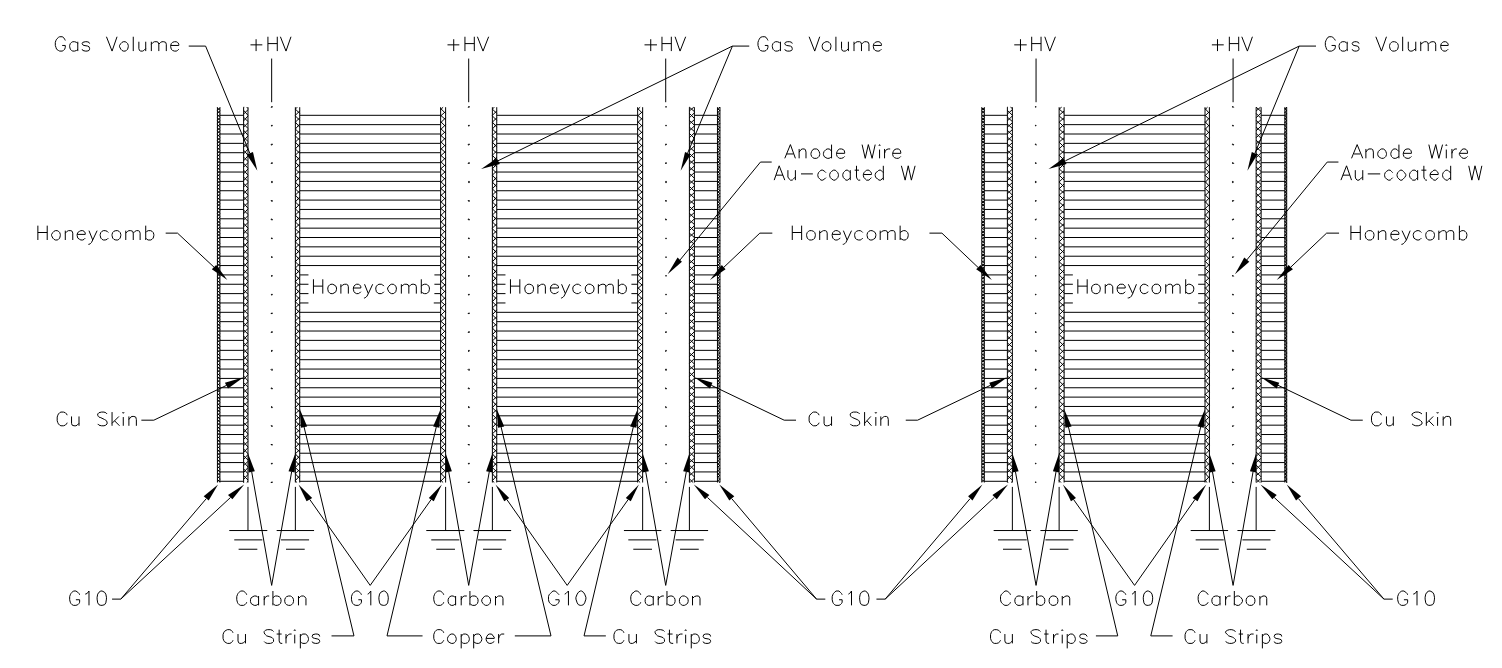
\includegraphics[width=0.8\textwidth]{figures/atlas/atlas_tgc_chamber.png}
    \caption{Cross section of a TGC triplet and doublet module. The triplet module consists of three planes of anodes, while the doublet module consists of two planes of anodes. Taken from~\cite{atlas_collaboration_paper}.}\label{fig:tgc_chamber}
\end{figure}

TGCs are multi-wire proportional chambers distinguished by a wire-to-cathode distance of 1.4 mm which is smaller than the wire-to-wire distance of 1.8 mm. This allows for excellent time resolution for most tracks. However, tracks that pass perpendicularly between the wires can have longer drift times due to the vanishing drift field. The chambers operate with a highly quenching gas mixture composed of 55\% $CO_2$ and 45\% of $n-C_5H_{12}$ allowing for operation in a quasi-saturated mode. TGC signals typically arrive within a 25 ns window with 99\% probability, allowing reliable bunch-crossing identification. The full TGC systems contains approximately 400,000 readout channels.
